\chapter{Kourabie}
\label{ch:kourabie}
\index{dessert}
\index{cookies}
\index{Christmas}

\marginnote{
    \textbf{Makes 25-30 cookies} \\
    Prep time: 45 minutes \\
    Cook time: 15-20 minutes \\
    \vspace*{\baselineskip}

    400g all-purpose flour \\
    250g butter, cold and cut into small cubes \\
    200g almonds, blanched whole \\
    1 tbsp baking powder \\
    75g icing sugar, sifted \\
    1 tbsp rosewater \\
    1/2 tsp vanilla extract \\
    1 pinch salt \\
    Icing sugar for powdering
}

\begin{figure}
  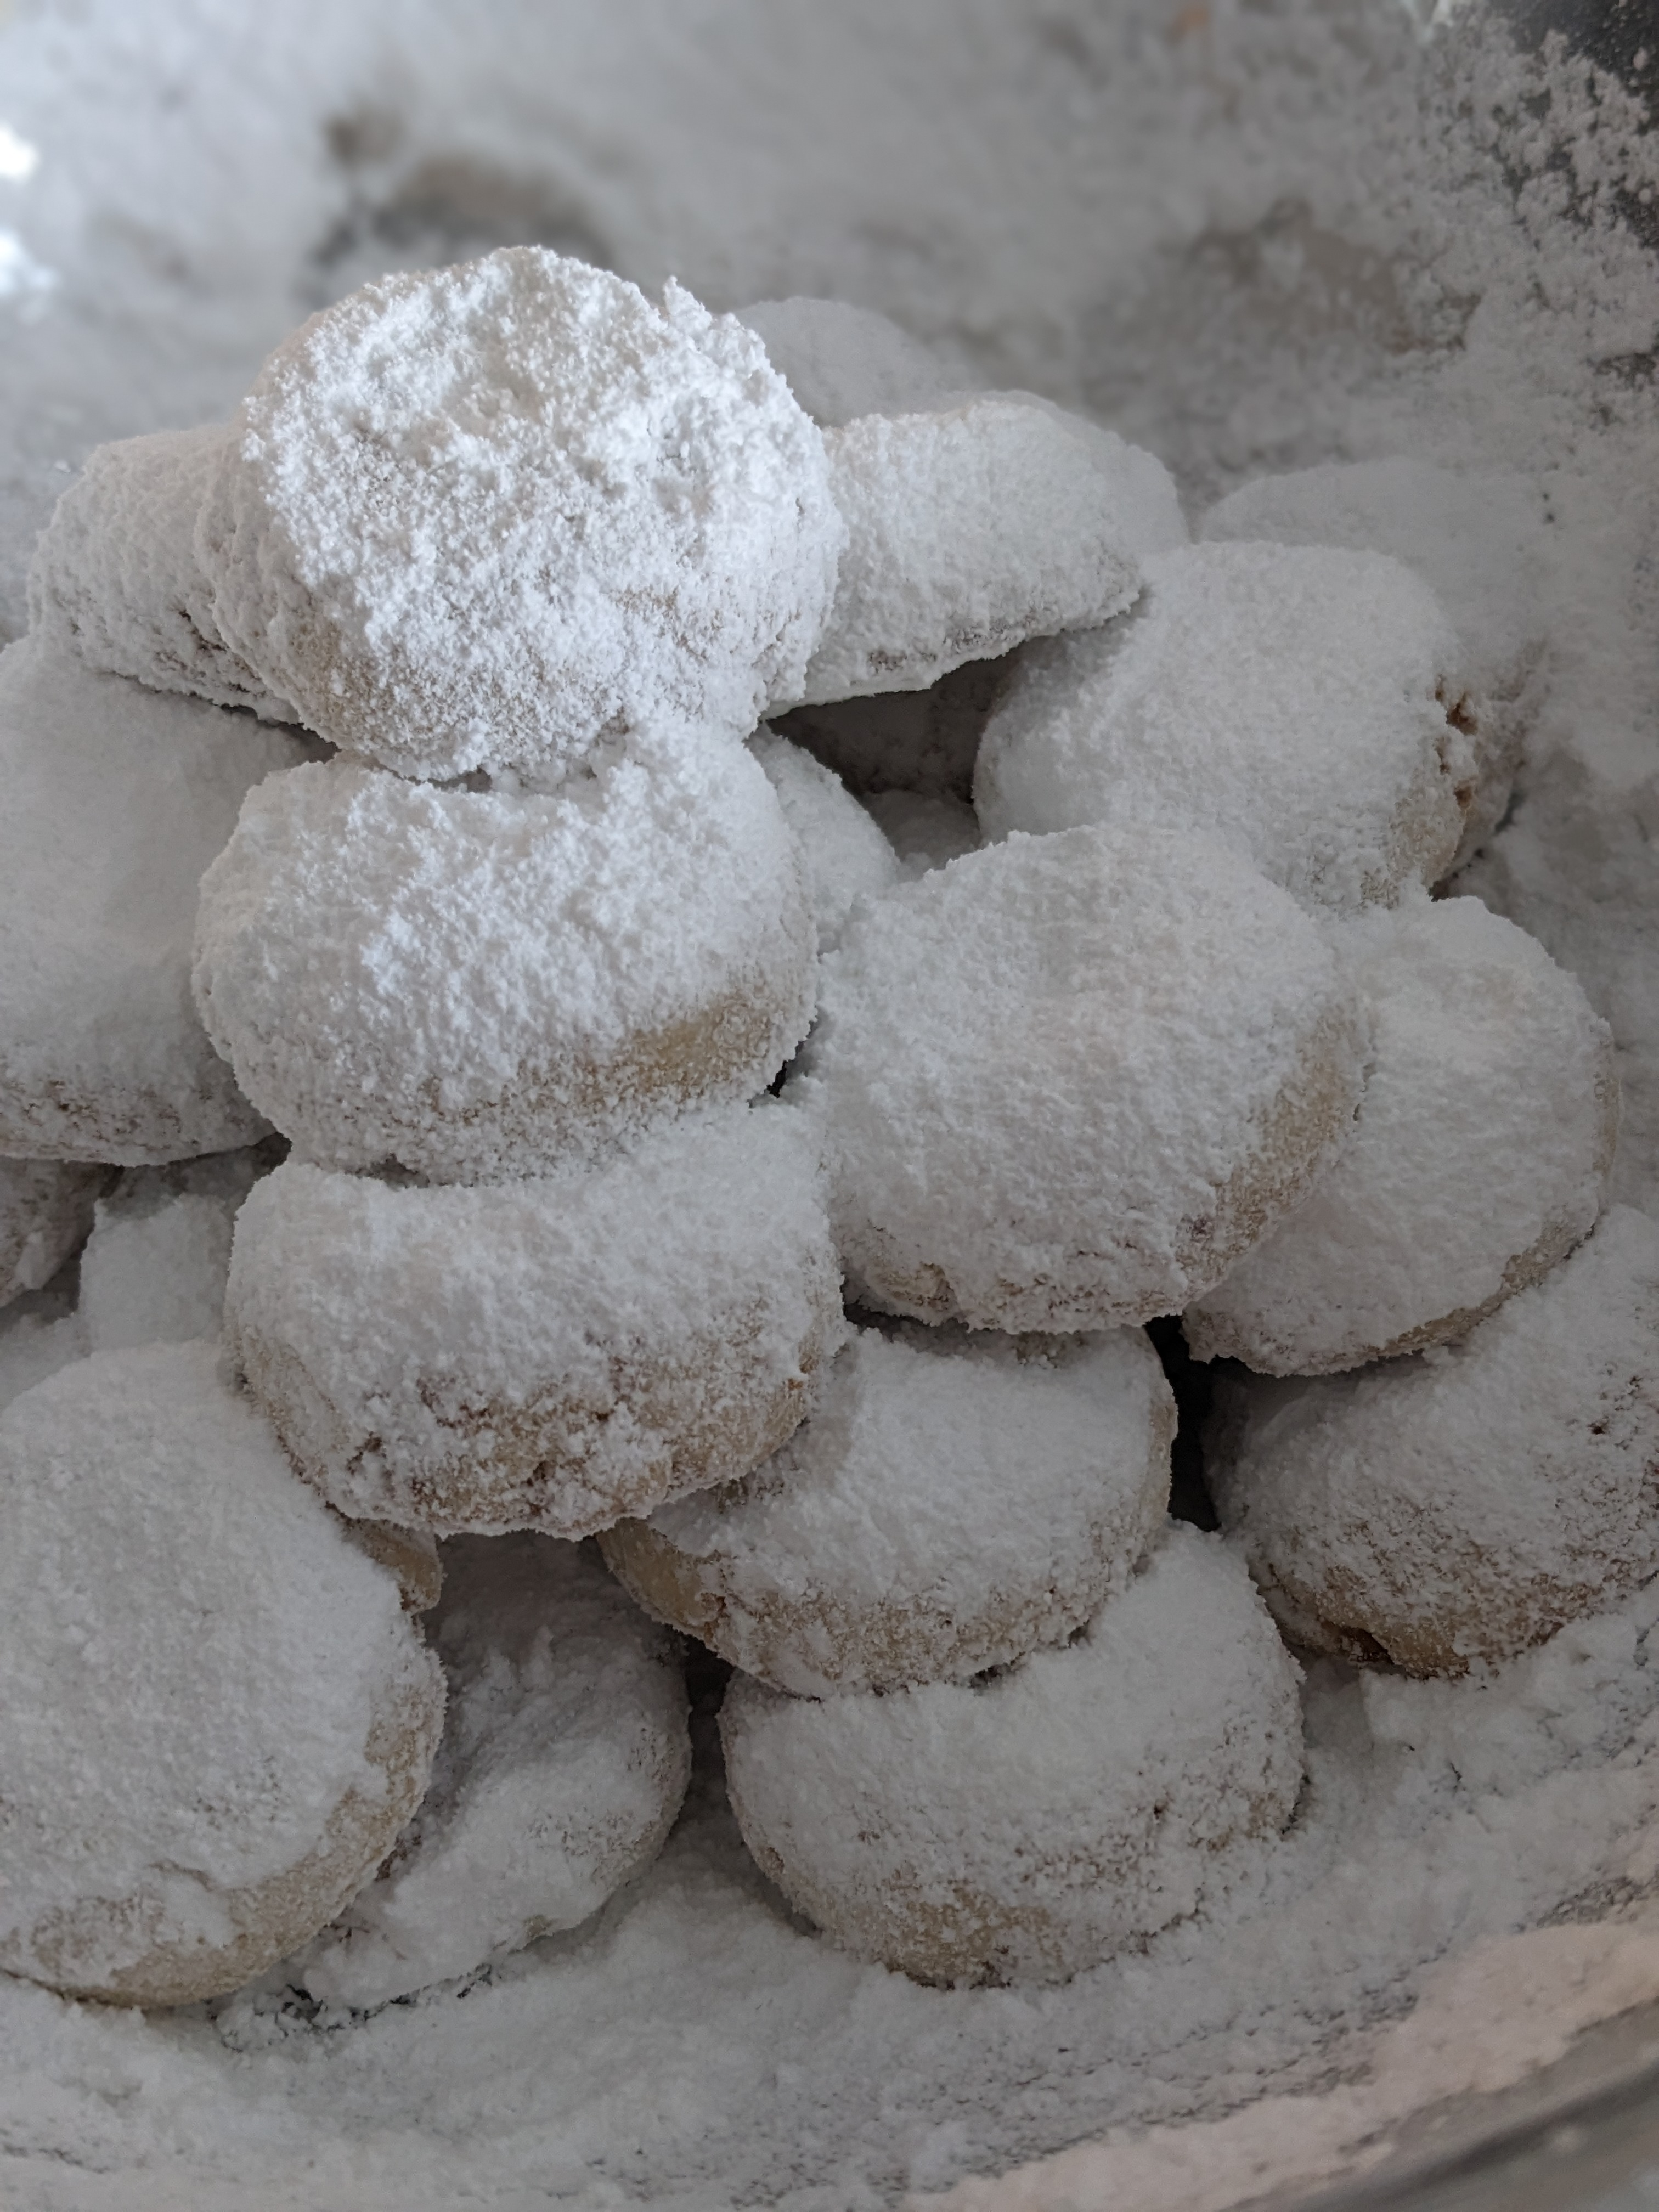
\includegraphics[width=60mm]{velsa/images/Kourabie.jpg}
\end{figure}

\textit{Shortbread cookies with powdered sugar and almonds}

Family member: Elsa \& Vaski

\begin{enumerate}
    \item Preheat oven to 400\degree F and toast 150g of the almonds for 7-8 minutes. Once completely cooled, pulse in a food processor until coarsely chopped and pieces remain so the cookies will be crunchy. Place them aside in a small bowl.
    \item In a food processor, add 50g of the raw almonds and blend until powdered. Set aside in another bowl.
    \item In the food processor, add the cold butter and powdered sugar. Mix for 10-15 seconds until the butter is reduced in size, almost the size of peas. Add the 50g raw powdered almonds, a pinch of salt, the rosewater and vanilla. Mix for 10-20 seconds to combine and scrape the sides. Add the baking powder and flour and mix again for 10-15 seconds.
    \item Place the mixture in a larger bowl, add the 150g toasted  chopped almonds and mix lightly with your hands.
    \item Preheat oven to 350\degree F and layer 2 baking sheets with parchment paper.
    \item Roll dough into 1 tbsp (30g) balls and place them on the baking sheets. Slightly put with your finger in the middle, to form a little dimple. Place in the fridge for 10-15 minutes before baking.
    \item Bake for 15-20 minutes until the cookies are faintly golden on the top and colored on the bottom. Be careful not to overbake them.
    \item Let them completely cool before dusting them with powdered sugar.
\end{enumerate}
